\documentclass[a4paper]{article}

\usepackage[czech]{babel} %https://github.com/michal-h21/biblatex-iso690
\usepackage[
   backend=biber      % if we want unicode 
  ,style=iso-numeric % or iso-numeric for numeric citation method          
  ,babel=other        % to support multiple languages in bibliography
  ,sortlocale=cs_CZ   % locale of main language, it is for sorting
  ,bibencoding=UTF8   % this is necessary only if bibliography file is in different encoding than main document
]{biblatex}

\usepackage[utf8]{inputenc}
\usepackage{fancyhdr}
\usepackage{amsmath}
\usepackage{amssymb}
\usepackage[left=2cm,right=2cm,top=2.5cm,bottom=2.5cm]{geometry}
\usepackage{graphicx}
\usepackage{pdfpages}
\usepackage{url}
\usepackage{multirow}
\usepackage{array}

\usepackage{siunitx}
\sisetup{locale = DE, separate-uncertainty = true}  %, separate-uncertainty = true    kdybych chtel +/-

\usepackage{float}
\newfloat{graph}{htbp}{grp}
\floatname{graph}{Graf}
\newfloat{tabulka}{htbp}{tbl}
\floatname{tabulka}{Tabulka}

\renewcommand{\thefootnote}{\roman{footnote}}

\pagestyle{fancy}
\lhead{Praktikum I - (VI) Studium reologického chování látek}
\rhead{Vladislav Wohlrath}
\author{Vladislav Wohlrath}

\bibliography{source}

\begin{document}

\begin{titlepage}
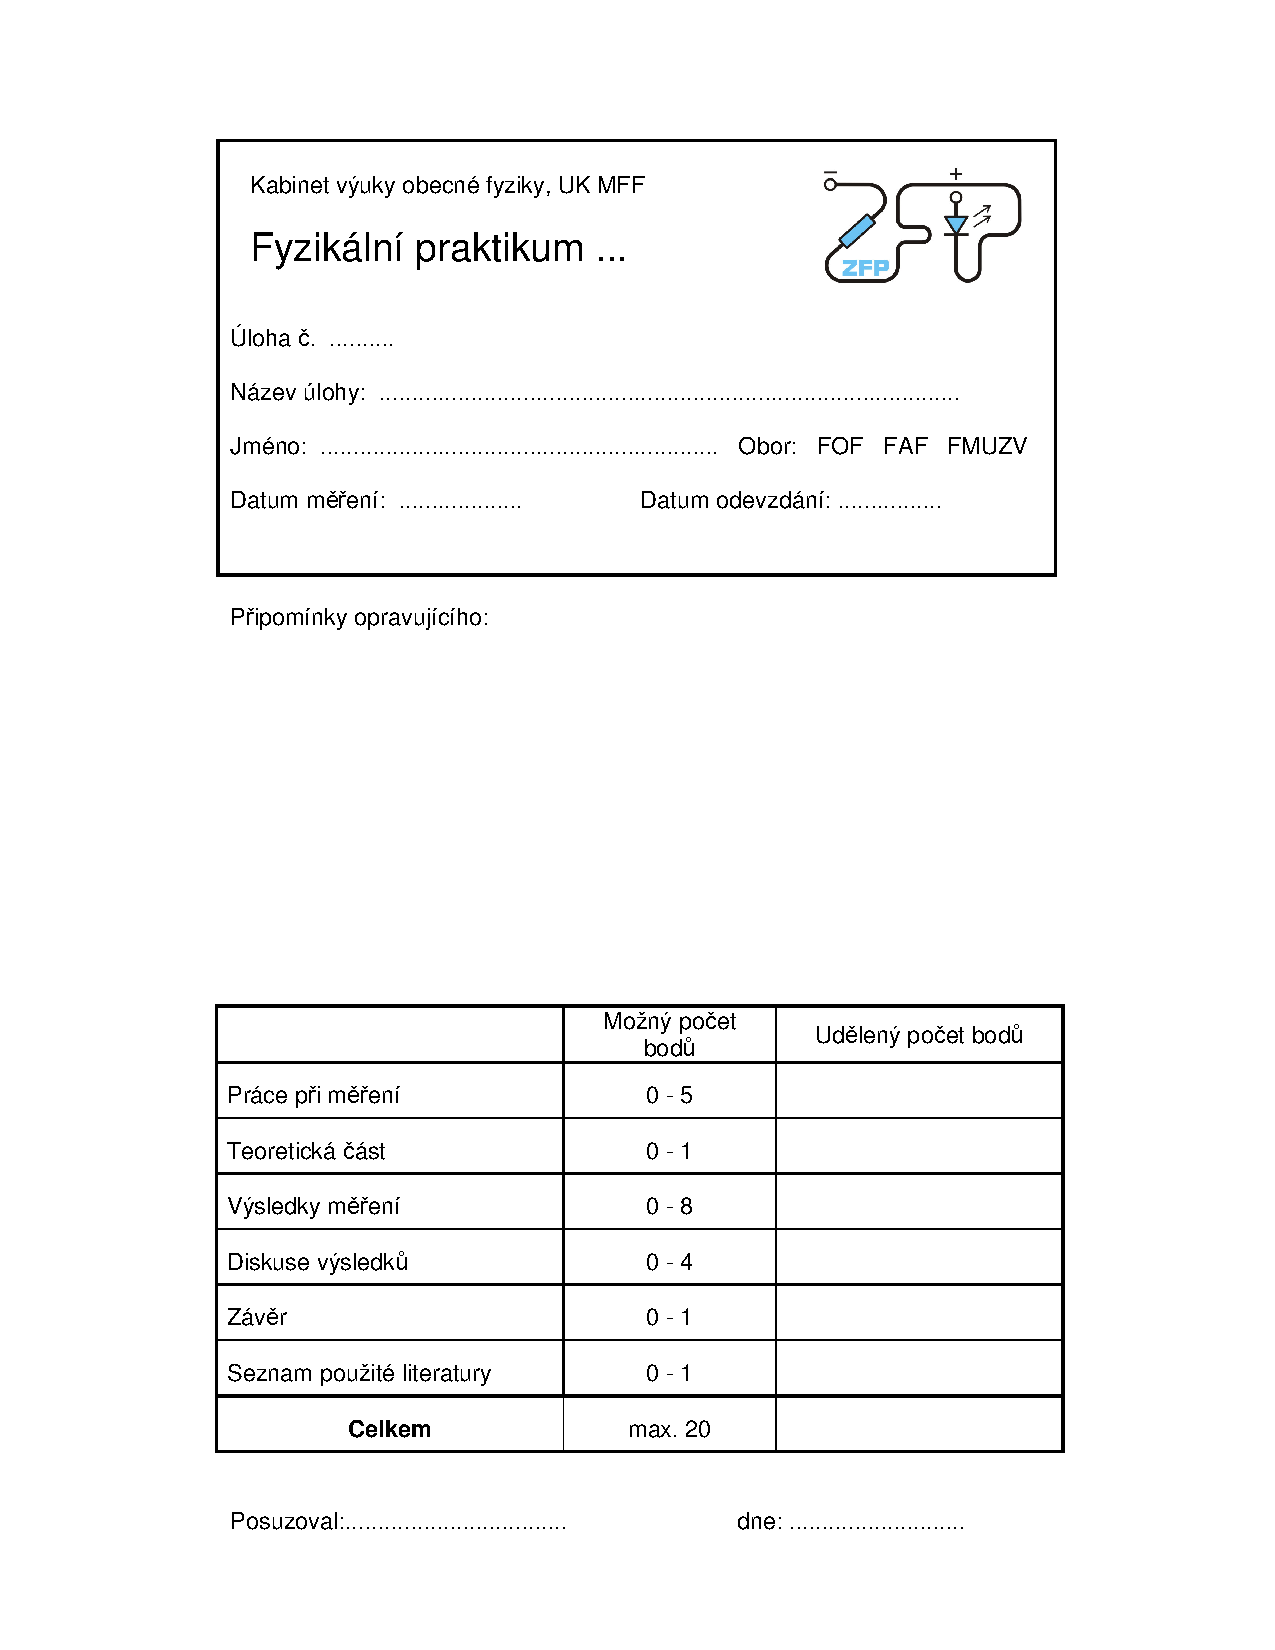
\includepdf[pages={1}]{./graficos/titlelist.pdf}
\end{titlepage}

\section*{Pracovní úkoly}
\begin{enumerate}
\item Měřením na rotačním viskozimetru zjistěte, zda jsou kapaliny připravené pro měření newtonovské.
\item Pomocí rotačního viskozimetru určete viskozitu newtonovské kapaliny.
\item Pro nenewtonovskou kapalinu změřte závislost zdánlivé viskozity na rychlosti otáčení rotoru a graficky znázorněte.
\item Změřte teplotní závislost viskozity glycerinu pomocí kuličkového viskozimetru v oboru teplot od \SI{25}{\degreeCelsius} do \SI{35}{\degreeCelsius}. Graficky znázorněte závislost $\eta = \eta(T)$. Určete aktivační energii.
\item Pyknometrickou metodou určete hustotu glycerinu a stanovte podíl vody v glycerinu. Změřenou viskozitu glycerinu srovnejte s tabelovanou hodnotou. 
\end{enumerate}

%Teoretická část
\section*{Teoretická část}
Dynamickou vikozitu kapaliny $\eta$ můžeme definovat vztahem \cite{skripta}
\begin{equation}
\tau = \eta \cdot D \,,
\end{equation}
kde $\tau$ je smykové napětí a $D$ je rychlost smykové deformace.

Pokud je $\eta$ konstanta a nezívisí na rychlosti deformace, nazýváme kapalinu newtonovskou.
Pokud $\eta$ na rychlosti závisí, mluvíme o zdánlivé viskozitě a kapalinu nazýváme nenewtonovskou.
Pro některé nenewtonovské kapaliny platí mocninný zákon \cite{skripta}
\begin{equation} \label{eq::fitnenewton}
\eta = m \cdot D^{n-1} \,,
\end{equation}
kde $m$ je konstanta a $n$ je číslo.

Změnu viskozity s teplotou můžeme charakterizovat vztahem \cite{skripta}
\begin{equation}
\eta(T) = C \cdot \exp(\frac{\epsilon_A}{kT}) \,,
\end{equation}
kde $C$ je konstanta, $\epsilon_A$ je aktivační energie, $k$ je Boltzmannova konstanta a $T$ je termodynamická teplota.
Po zlogaritmování dostaneme
\begin{equation} \label{eq::primka}
\ln(\eta) = \ln(C) + \frac{\epsilon_A}{k} \cdot \frac{1}{T} \,,
\end{equation}
tedy rovnici přímky v proměnných $\ln{\eta}$ a $1/T$.

Viskozitu budeme měřit rotačním a kuličkovým viskozimetrem značky HAAKE.

Rotační viskozimetr je vybaven čtyřmi rotory různé velikosti ozančenými \emph{L1}, \emph{L2}, \emph{L3} a \emph{L4} a umožňuje volit frekvenci otáčení.

V kuličkovém viskozimetru měříme čas $t$, za který kulička ve viskózní kapalině urazí vzdálenost \SI{100}{\mm}.
Kuličkový viskozimetr je připojen k přístroji, který umožňuje nastavit teplotu kapaliny.
Viskozitu určíme ze změřeného času $t$ pomocí vztahu \cite{skripta}
\begin{equation} \label{eq::teplotavypocet}
\eta = K \cdot (\rho_1 - \rho_2) \cdot t \,,
\end{equation}
kde $\rho_1$ je hustota kuličky, $\rho_2$ hustota kapaliny a $K$ je konstanta kuličky.
Byla použita ocelová kulička o hmotnosti \SI{14.92}{\g}, průměru \SI{15.19}{mm} a hustotě $\rho_1 = $\SI{8.127}{\g\per\cm\cubed}.
Pro takovou kuličku uvádí \cite{skripta} konstantu kuličky \mbox{$K = \SI{0.7061}{\milli\Pa\per\cm\cubed\per\g}$}.

Viskozita glycerinu je silně závislá na složení a v rotačním viskozimetru neměříme čistý glycerin.
Jeho koncentraci změříme pyknometrickou metodou \cite{pyknometr}.
Změříme hmotnost prázdného pyknometru $m_1$, hmotnost pyknometru naplněného vodou (o známé hustotě) $m_2$ a hmotnost pyknometru naplněného glycerinem $m_3$.
Hustotu glycerinu určíme podle vztahu \cite{skripta}
\begin{equation} \label{eq::pyknometr}
\rho_{glycerin} = \frac{m_3 - m_1}{m_2 - m_1} \cdot (\rho_{voda} - \sigma) + \sigma \,,
\end{equation}
kde $\sigma$ je hustota vzduchu.

%Podmínky a měřící přístroje
%\section*{Podmínky}


%Výsledky měření
\section*{Výsledky měření}

%Diskuze výsledků
\section*{Diskuze}

%Závěr
\section*{Závěr}


\printbibliography[title={Seznam použité literatury}]

\end{document}